\documentclass{article}
\usepackage{amsmath}
\usepackage[margin=0.5in]{geometry}
\usepackage{hyperref}
\usepackage{graphicx}
\graphicspath{ {.} }

\title{CAP6617 Project}
\date{13 December 2016}
\author{Jennifer Cheung and Armand Kapllani}
\begin{document}
	\maketitle
	\textbf{Choice of dataset:}  To run the linear classifier, we restricted the dataset to the training set of the Kaggle images because they were labeled. I'm not masochistic enough to go through each image and label them cat or dog in the test file. \\
	The training set were chosen using a uniform distribution via the matlab datasample() method. \\  
	We're using 12,000 out of the 25,000 samples due to the processing time (Each run of the classifier takes ~30 min) that have been resized to 250 $\times$ 250.  For the extra credit, we threw in 4,500 images of birds, removing the images which don't have rgb fields.

	\section{Results using trained CNN and linear Kernal SVM}
	\subsection{20\% training}
	\begin{enumerate}
		\item kFold CV accuracy: 0.9112  \indent Test Set accuracy: 0.9153
		\item kFold CV accuracy: 0.9146  \indent Test Set accuracy: 0.9189
		\item kFold CV accuracy: 0.9021  \indent Test Set accuracy: 0.9087
		\item kFold CV accuracy: 0.9158  \indent Test Set accuracy: 0.9197
		\item kFold CV accuracy: 0.9129  \indent Test Set accuracy: 0.9173
	\end{enumerate}

	\textbf{Average:} Crossvalidation Accuracy: 0.9113;  Test Set Accuracy: 0.9160

	\subsection{15\% training}
	\begin{enumerate}
		\item kFold CV accuracy: 0.9061  \indent Test Set accuracy: 0.9075
		\item kFold CV accuracy: 0.9050  \indent Test Set accuracy: 0.9089
		\item kFold CV accuracy: 0.8956  \indent Test Set accuracy: 0.9088
		\item kFold CV accuracy: 0.9044  \indent Test Set accuracy: 0.9129
		\item kFold CV accuracy: 0.9033  \indent Test Set accuracy: 0.9101
	\end{enumerate}

	\textbf{Average:} Crossvalidation Accuracy: 0.9029;  Test Set Accuracy: 0.9097

	\subsection{10\% training}
	\begin{enumerate}
		\item kFold CV accuracy: 0.8992  \indent Test Set accuracy: 0.8910
		\item kFold CV accuracy: 0.8883  \indent Test Set accuracy: 0.8979
		\item kFold CV accuracy: 0.9100  \indent Test Set accuracy: 0.8952
		\item kFold CV accuracy: 0.8758  \indent Test Set accuracy: 0.8975
		\item kFold CV accuracy: 0.9100  \indent Test Set accuracy: 0.8870
	\end{enumerate}

	\textbf{Average:} Crossvalidation Accuracy: 0.8967;  Test Set Accuracy: 0.8937

	\subsection{5\% training}
	\begin{enumerate}
		\item kFold CV accuracy: 0.8850  \indent Test Set accuracy: 0.8660
		\item kFold CV accuracy: 0.8883  \indent Test Set accuracy: 0.8844
		\item kFold CV accuracy: 0.9033  \indent Test Set accuracy: 0.8939
		\item kFold CV accuracy: 0.8750  \indent Test Set accuracy: 0.8929
		\item kFold CV accuracy: 0.8950  \indent Test Set accuracy: 0.8854
	\end{enumerate}

	\textbf{Average:} Crossvalidation Accuracy: 0.8893;  Test Set Accuracy: 0.8845

	\subsection{1\% training}
	\begin{enumerate}
		\item kFold CV accuracy: 0.7917  \indent Test Set accuracy: 0.8144
		\item kFold CV accuracy: 0.8417  \indent Test Set accuracy: 0.8158
		\item kFold CV accuracy: 0.8583  \indent Test Set accuracy: 0.8216
		\item kFold CV accuracy: 0.8250  \indent Test Set accuracy: 0.7739
		\item kFold CV accuracy: 0.8417  \indent Test Set accuracy: 0.8854
	\end{enumerate}

	\textbf{Average:} Crossvalidation Accuracy: 0.8317;  Test Set Accuracy: 0.8222
	\\ \\

	\centerline{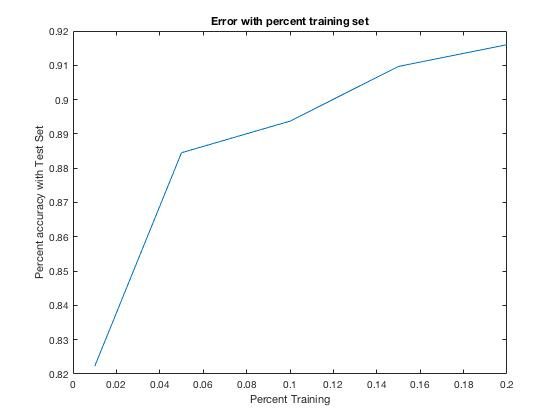
\includegraphics[scale=0.35]{errorgraph}} 

	\section{Results using trained CNN and linear Kernal SVM with additional Bird dataset}
	\subsection{20\% training}
	\begin{enumerate}
		\item kFold CV accuracy: 0.9015  \indent Test Set accuracy: 0.8981
		\item kFold CV accuracy: 0.9045  \indent Test Set accuracy: 0.8992
		\item kFold CV accuracy: 0.8976  \indent Test Set accuracy: 0.9076
		\item kFold CV accuracy: 0.9106  \indent Test Set accuracy: 0.9038
		\item kFold CV accuracy: 0.9121  \indent Test Set accuracy: 0.9170
	\end{enumerate}

	\textbf{Average:} Crossvalidation Accuracy: 0.9053;  Test Set Accuracy: 0.9052

	\subsection{15\% training}
	\begin{enumerate}
		\item kFold CV accuracy: 0.8893  \indent Test Set accuracy: 0.8916
		\item kFold CV accuracy: 0.9156  \indent Test Set accuracy: 0.8952
		\item kFold CV accuracy: 0.8937  \indent Test Set accuracy: 0.8895
		\item kFold CV accuracy: 0.8958  \indent Test Set accuracy: 0.9012
		\item kFold CV accuracy: 0.8945  \indent Test Set accuracy: 0.8977
	\end{enumerate}

	\textbf{Average:} Crossvalidation Accuracy: 0.8978;  Test Set Accuracy: 0.8950

	\subsection{10\% training}
	\begin{enumerate}
		\item kFold CV accuracy: 0.8885  \indent Test Set accuracy: 0.8673
		\item kFold CV accuracy: 0.8927  \indent Test Set accuracy: 0.8721
		\item kFold CV accuracy: 0.9006  \indent Test Set accuracy: 0.8768
		\item kFold CV accuracy: 0.8758  \indent Test Set accuracy: 0.8801
		\item kFold CV accuracy: 0.8964  \indent Test Set accuracy: 0.8845
	\end{enumerate}

	\textbf{Average:} Crossvalidation Accuracy: 0.8908;  Test Set Accuracy: 0.9052

	\subsection{5\% training}
	\begin{enumerate}
		\item kFold CV accuracy: 0.8679  \indent Test Set accuracy: 0.8378
		\item kFold CV accuracy: 0.8679  \indent Test Set accuracy: 0.8536
		\item kFold CV accuracy: 0.8691  \indent Test Set accuracy: 0.8539
		\item kFold CV accuracy: 0.8836  \indent Test Set accuracy: 0.8686
		\item kFold CV accuracy: 0.8945  \indent Test Set accuracy: 0.8718
	\end{enumerate}

	\textbf{Average:} Crossvalidation Accuracy: 0.8766;  Test Set Accuracy: 0.8591

	\subsection{1\% training}
	\begin{enumerate}
		\item kFold CV accuracy: 0.7455  \indent Test Set accuracy: 0.6479
		\item kFold CV accuracy: 0.7939  \indent Test Set accuracy: 0.5924
		\item kFold CV accuracy: 0.8121  \indent Test Set accuracy: 0.7011
		\item kFold CV accuracy: 0.8667  \indent Test Set accuracy: 0.6079
		\item kFold CV accuracy: 0.7333  \indent Test Set accuracy: 0.5936
	\end{enumerate}

	\textbf{Average:} Crossvalidation Accuracy: 0.7903;  Test Set Accuracy: 0.6286
	\\ \\

	\centerline{\includegraphics[scale=0.45]{errorgraphwithbirds}}

	\section{Code and Files}
	\setlength\parindent{34pt} \href{https://github.com/jenncheung/Advance-Machine-Learning-Project}{Code on Jennifer's github: http://www.vision.caltech.edu/visipedia/CUB-200-2011.html} \\
	\href{http://www.vision.caltech.edu/visipedia/CUB-200-2011.html}{Birds Dataset ripped from caltech: http://www.vision.caltech.edu/visipedia/CUB-200-2011.html}\\
	\textbf{Datasets:} \href{https://www.dropbox.com/s/hz1h63s8ru5ug1p/Datasets.zip?dl=0}{https://www.dropbox.com/s/hz1h63s8ru5ug1p/Datasets.zip?dl=0}\\
	\textbf{Just for funsies:} \\
	I put in the \href{http://guardianlv.com/wp-content/uploads/2014/05/The-Panda-Dog-Is-the-Newest-Rage-in-China.jpg}{PANDADOG (click here)} to see what would happen, and it reads back correctly as a dog.  Which probably means that all pandas will read back as dogs, even though this is actually a dog, seriously though, look at the pandadog, it's super cute.
\end{document}